\documentclass{beamer}
\usepackage[utf8]{inputenc}
\usepackage[spanish]{babel}
\usepackage{hyperref}
\usepackage{verbatim}
\usepackage{listings}

\setbeamercovered{invisible}
\usetheme{Frankfurt}

% Configurar los listings (Códigos)
\renewcommand{\lstlistingname}{Código}
\lstset{
	language=C++,               % Lenguaje
	basicstyle=\ttfamily\tiny,  % Tipo de fuente
	keywordstyle=\color{blue},  % Color de palabras clave
	stringstyle=\color{red},    % Color de strings
	commentstyle=\color{gray},  % Color de comentarios
	showstringspaces=false,     % No muestrar el _ cuando el string tiene espacios
	breaklines = true,          % Partir las líneas largas
	breakatwhitespace=true,	    % Partir las líneas en un espacio
	numbers=left,				% Numerar las líneas a la izq
	numberstyle=\tiny,			% Poner los números de las líneas pequeños
	numberblanklines=true,      % Numerar las líneas en blanco
	columns=fullflexible,       % No perder el formato al dejar los espacios
	keepspaces=true,   			% Dejar los espacios insertados
	frame=tb,					% Poner el recuadro
}


\title{Semillero de Programación}
\author{Ana Echavarría \and Juan Francisco Cardona}

\institute{Universidad EAFIT}
\date{\today}

\begin{document}

\begin{frame}
	\titlepage
\end{frame}

\begin{frame}
	\frametitle{Contenido}
	\tableofcontents
\end{frame}


\begin{section}{Arreglos de C++}
	\begin{frame}[fragile]
		\frametitle{Arreglos de C++}
		\begin{itemize}
			\item{Un arreglo es una serie de elementos del mismo tipo ordenados en una secuencia lineal.}
			\item{El número de elementos del arreglo es fijo.}
			\item{Se puede acceder a cada elemento de manera individual usando el índice de su posición, empezando por el índice 0.}
			\item{Por ejemplo, un arreglo de 10 posiciones llamado $a$ puede ser representado así:}
			\begin{figure}
				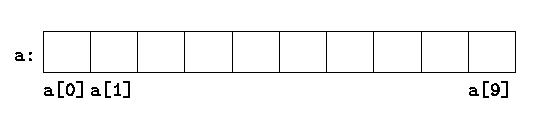
\includegraphics[width = 0.7\textwidth]{arreglo.jpg}
			\end{figure}			
		\end{itemize}
	\end{frame}
	
	\begin{frame}[fragile]
		\frametitle{Arreglos de C++}
		Un arreglo debe ser declarado antes de usarse. Para declararse se hace lo siguiente.
		\begin{block}{Declaración de arreglos}
			\begin{verbatim}
				tipo_de_dato nombre [número_de_elementos];
			\end{verbatim}
			Ejemplos:\\
			\begin{verbatim}
				int a [10];
				string palabras [50];
			\end{verbatim}			
		\end{block}		
	\end{frame}
	
	\begin{frame}[fragile]
		\frametitle{Arreglos de C++}
		Se pueden declarar arreglos de varias dimensiones
		\begin{block}{Arreglos de varias dimensiones}
			\begin{verbatim}
				tipo_de_dato nombre [tam_dim_1] ... [tam_dim_n];
			\end{verbatim}
			Ejemplo:
			\begin{verbatim}
				int jimmy [3][5];
			\end{verbatim}	
		\end{block}
		\begin{figure}
			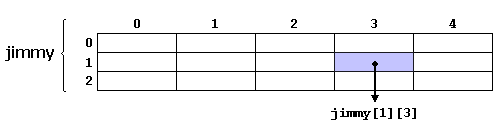
\includegraphics[width = 0.8\textwidth]{arreglo2.png}
		\end{figure}		
	\end{frame}
	
	\begin{frame}[fragile]
		\frametitle{Arreglos de C++}
		\small{El problema Next Round se puede resolver usando arreglos (http://www.codeforces.com/problemset/problem/158/A)}
		\begin{lstlisting}
			using namespace std;
			#include <iostream>

			const int MAXN = 55;
			int a [MAXN];

			int main(){
			    int n, k;
			    cin >> n >> k;
			    for (int i = 0; i < n; i++) cin >> a[i];

			    int count = 0;
			    int min_score = a[k-1];
			    for (int i = 0; i < n; i++){
			        if (a[i] >= min_score and a[i] > 0) count++;
			        else break;
			    }
			    cout << count << endl;
			    
				return 0;
			}
		\end{lstlisting}		
	\end{frame}	
\end{section}

\begin{section}{Vectores de C++}
	\begin{frame}[fragile]
		\frametitle{Vectores de C++}
		\begin{itemize}
			\item {Los vectores son contenedores que almacenan los datos en una secuencia pero que pueden cambiar de tamaño.}
			\item {Al igual que los arreglos, los elementos pueden ser accedidos por medio del índice de su posición, empezando por en índice 0.}
			\item {Contrario a los arreglos, el tamaño de los vectores cambia dinámicamente. Esto hace que utilicen más memoria para poder crecer eficientemente.}
		\end{itemize}
		\begin{figure}
			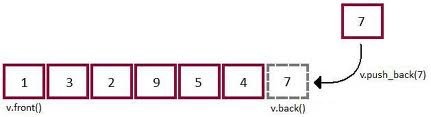
\includegraphics[width = 0.8\textwidth]{vector.jpg}
		\end{figure}
	\end{frame}
	
	\begin{frame}[fragile]
		\frametitle{Vectores de C++}
		Para utilizar un arreglo es necesario incluir la librería vector.\\
		\verb|#include <vector> |
		\begin{block}{Declaración de vector}
			\begin{verbatim}
				vector <tipo_de_dato> nombre;
			\end{verbatim}
			Ejemplos:\\
			\begin{verbatim}
				vector <int> a;
				vector <string> palabras (50);
				vector <int> zeros (500, 0);
			\end{verbatim}			
		\end{block}		
	\end{frame}
	
	\begin{frame}[fragile]
		\frametitle{Vectores de C++}
		\small{El problema Next Round se puede resolver usando arreglos (http://www.codeforces.com/problemset/problem/158/A)}
		\begin{lstlisting}
			using namespace std;
			#include <iostream>
			#include <vector>

			vector <int> a;

			int main(){
			    int n, k;
			    cin >> n >> k;
			    a.clear();
			    for (int i = 0; i < n; i++){
			        int ai;
			        cin >> ai;
			        a.push_back(ai); 
			    }

			    int count = 0;
			    int min_score = a[k-1];
			    for (int i = 0; i < n; i++){
			        if (a[i] >= min_score and a[i] > 0) count++;
			        else break;
			    }
			    cout << count << endl;
			    
				return 0;
			}
		\end{lstlisting}		
	\end{frame}
	
	\begin{frame}[fragile]
		\frametitle{Arreglos y vectores en C++}
		\begin{alertblock}{Pregunta}
			¿Qué significa \verb|vector <int> g [1000]|? 
		\end{alertblock}\pause
		\begin{exampleblock}{Respuesta}
			Es un arreglo de 1000 posiciones en el que cada posición contiene un vector de enteros
		\end{exampleblock}
	\end{frame}	
\end{section}

\begin{section}{Grafos}
	\begin{frame}
		\frametitle{Grafos dirigidos}
		Un grafo dirigido $G$ es un par $(V, E)$ donde $V$ es un conjunto finito de \textbf{nodos} (vertices) y $E$ es un conjunto de \textbf{parejas ordenadas} donde cada elemento es un elemento de $V$ y es llamado conjunto de \textbf{aristas} (edges).\\
		En la siguiente figura $V = \{1, 2, 3, 4, 5, 6\}$ y $E = \{(1, 2), (2, 2), (2, 4), (2, 5), (4, 1), (4, 5), (5, 4), (6, 3)\}$
		\begin{figure}
			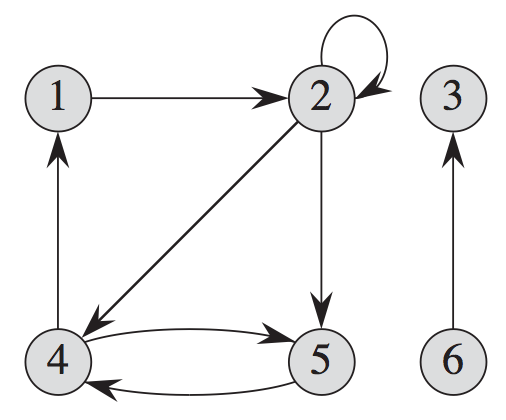
\includegraphics[height = 0.35\textheight]{digraph.png}
		\end{figure}		
	\end{frame}
	
	\begin{frame}
		\frametitle{Grafos no dirigidos}
		En un grafo dirigido $G = (V, E)$, $V$ es un conjunto finito de \textbf{nodos} (vertices) y $E$ es un conjunto de \textbf{parejas no ordenadas} $(u, v)$ donde $u, v \in V$ y $u \ne v$.\\
		En la siguiente figura $V = \{1, 2, 3, 4, 5, 6\}$ y $E = \{(1, 2), (1, 5), (2, 5), (6, 3)\}$
		\begin{figure}
			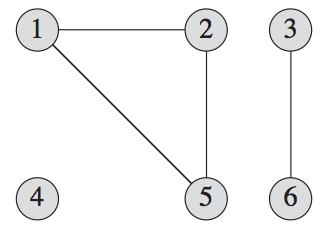
\includegraphics[height = 0.35\textheight]{graph.png}
		\end{figure}		
	\end{frame}
	
	\begin{frame}
		\frametitle{Representación de grafos}
		
		
	\end{frame}
	
\end{section}

\end{document}